\subsection{Slučaj upotrebe: Definisanje faza produkcije}

\subsubsection*{Kratak opis}

Projektni menadžer za projekat animiranog filma definiše faze produkcije i njihov redosled, uz odgovorni tim za svaku fazu. Definisane faze koriste se za planiranje budžeta i rokova, pa se producent obaveštava o njihovom definisanju i promenama.

\subsubsection*{Akteri}
\begin{itemize}
    \item \textbf{Projektni menadžer} -- definiše faze produkcije, menja ih i određuje njihov redosled.
    \item \textbf{Producent} -- prima obaveštenja o definisanim ili izmenjenim fazama, jer za njih planira budžet i rokove.
\end{itemize}

\subsubsection*{Preduslovi}
\begin{itemize}
    \item Projektni menadžer je prijavljen na sistem i angažovan na projektu.
    \item Projekat animiranog filma postoji u sistemu.
\end{itemize}

\subsubsection*{Postuslovi}
\begin{itemize}
    \item Faze produkcije su sačuvane u sistemu sa redosledom i odgovornim timom, a svaka izmena je zabeležena sa autorom i datumom.
    \item Ako su faze definisane ili izmenjene, producent je obavešten.
\end{itemize}

\subsubsection*{Osnovni tok}
\begin{enumerate}
    \item Projektni menadžer bira projekat i opciju ,,Faze produkcije''.
    \item Sistem prikazuje listu faza projekta i opciju ,,Dodaj fazu''.
    \item Projektni menadžer bira opciju ,,Dodaj fazu'' i unosi podatke o fazi.
    \item Sistem proverava podatke i dodaje fazu u redosled faza projekta. Koraci 3 i 4 se ponavljaju dok projektni menadžer ne unese sve faze.
    \item Po potrebi, projektni menadžer menja faze: izmena podataka faze (podtok P1), promena redosleda faza (podtok P2) ili brisanje faze (podtok P3).
    \item Projektni menadžer bira opciju ,,Potvrdi faze''.
    \item Sistem čuva definisane faze, obaveštava producenta i prikazuje poruku o uspešnom čuvanju.
\end{enumerate}

\subsubsection*{Podtokovi}

\paragraph*{P1: Izmena podataka faze}
\begin{enumerate}
    \item Projektni menadžer bira fazu i opciju ,,Izmeni fazu''.
    \item Projektni menadžer menja podatke o fazi i potvrđuje.
    \item Sistem proverava podatke i ažurira fazu.
\end{enumerate}
Podtok se poziva iz koraka 5 osnovnog toka, a po završetku se nastavlja od koraka 5.

\paragraph*{P2: Promena redosleda faza}
\begin{enumerate}
    \item Projektni menadžer bira fazu i opciju za pomeranje, ili unosi novi redni broj faze.
    \item Sistem menja redosled i ponovo numeriše faze.
\end{enumerate}
Podtok se poziva iz koraka 5 osnovnog toka, a po završetku se nastavlja od koraka 5.

\paragraph*{P3: Brisanje faze}
\begin{enumerate}
    \item Projektni menadžer bira fazu i opciju ,,Obriši fazu''.
    \item Sistem traži potvrdu, a projektni menadžer potvrđuje.
    \item Sistem briše fazu i ponovo numeriše preostale faze.
\end{enumerate}
Podtok se poziva iz koraka 5 osnovnog toka, a po završetku se nastavlja od koraka 5.

\subsubsection*{Alternativni tokovi}

\paragraph*{A1: Nepopunjena ili neispravna polja}
\begin{itemize}
    \item \textbf{Izaziva ga:} korak 4 osnovnog toka i korak 3 podtoka P1, ako neko obavezno polje nije popunjeno ili je neispravno.
    \item \textbf{Ispravka:}
    \begin{enumerate}
        \item Sistem označava neispravna polja i prikazuje poruku o grešci.
        \item Projektni menadžer ispravlja podatke i ponovo potvrđuje unos.
    \end{enumerate}
    \item \textbf{Povratak:} na korak 3 osnovnog toka (ako je izazvan korakom 4), odnosno na korak 2 podtoka P1.
\end{itemize}

\paragraph*{A2: Faza sa istim nazivom već postoji}
\begin{itemize}
    \item \textbf{Izaziva ga:} korak 4 osnovnog toka i korak 3 podtoka P1, ako projekat već ima fazu sa istim nazivom.
    \item \textbf{Ispravka:}
    \begin{enumerate}
        \item Sistem obaveštava projektnog menadžera da naziv faze već postoji.
        \item Projektni menadžer unosi drugačiji naziv.
    \end{enumerate}
    \item \textbf{Povratak:} na korak 3 osnovnog toka, odnosno na korak 2 podtoka P1.
\end{itemize}

\paragraph*{A3: Projekat već ima definisane faze}
\begin{itemize}
    \item \textbf{Izaziva ga:} korak 2 osnovnog toka, ako su faze projekta već definisane.
    \item \textbf{Ispravka:}
    \begin{enumerate}
        \item Sistem prikazuje postojeće faze sa njihovim redosledom i odgovornim timovima.
        \item Projektni menadžer po potrebi dodaje nove faze (koraci 3 i 4).
    \end{enumerate}
    \item \textbf{Povratak:} na korak 5 osnovnog toka.
\end{itemize}

\paragraph*{A4: Faza se ne može obrisati}
\begin{itemize}
    \item \textbf{Izaziva ga:} korak 3 podtoka P3, ako faza ima dodeljene zadatke ili evidentirane troškove.
    \item \textbf{Ispravka:}
    \begin{enumerate}
        \item Sistem ne briše fazu i prikazuje poruku da je faza u upotrebi.
    \end{enumerate}
    \item \textbf{Povratak:} na korak 5 osnovnog toka.
\end{itemize}

\paragraph*{A5: Odustajanje}
\begin{itemize}
    \item \textbf{Izaziva ga:} bilo koji korak osnovnog toka ili podtokova, ako projektni menadžer odustane.
    \item \textbf{Ispravka:}
    \begin{enumerate}
        \item Sistem odbacuje nesačuvane izmene i vraća projektnog menadžera na stranicu projekta.
    \end{enumerate}
    \item \textbf{Povratak:} nema povratka, slučaj upotrebe se završava.
\end{itemize}

\subsubsection*{Specijalni zahtevi}
\begin{itemize}
    \item Naziv faze je jedinstven u okviru projekta, a redni brojevi faza se ne ponavljaju.
    \item Faza koja ima dodeljene zadatke ili evidentirane troškove ne sme se obrisati.
\end{itemize}

\subsubsection*{Dodatne informacije}
\begin{itemize}
    \item Uobičajene faze produkcije: razvoj ideje, scenario, dizajn likova i okruženja, animacija, montaža, postprodukcija i distribucija.
    \item Polja formulara za fazu: naziv faze, opis, redni broj, odgovorni tim.
    \item Budžet i rokovi faza određuju se u slučaju upotrebe ,,Upravljanje budžetom i rokovima''.
\end{itemize}


\begin{figure}[H]
	\centering
	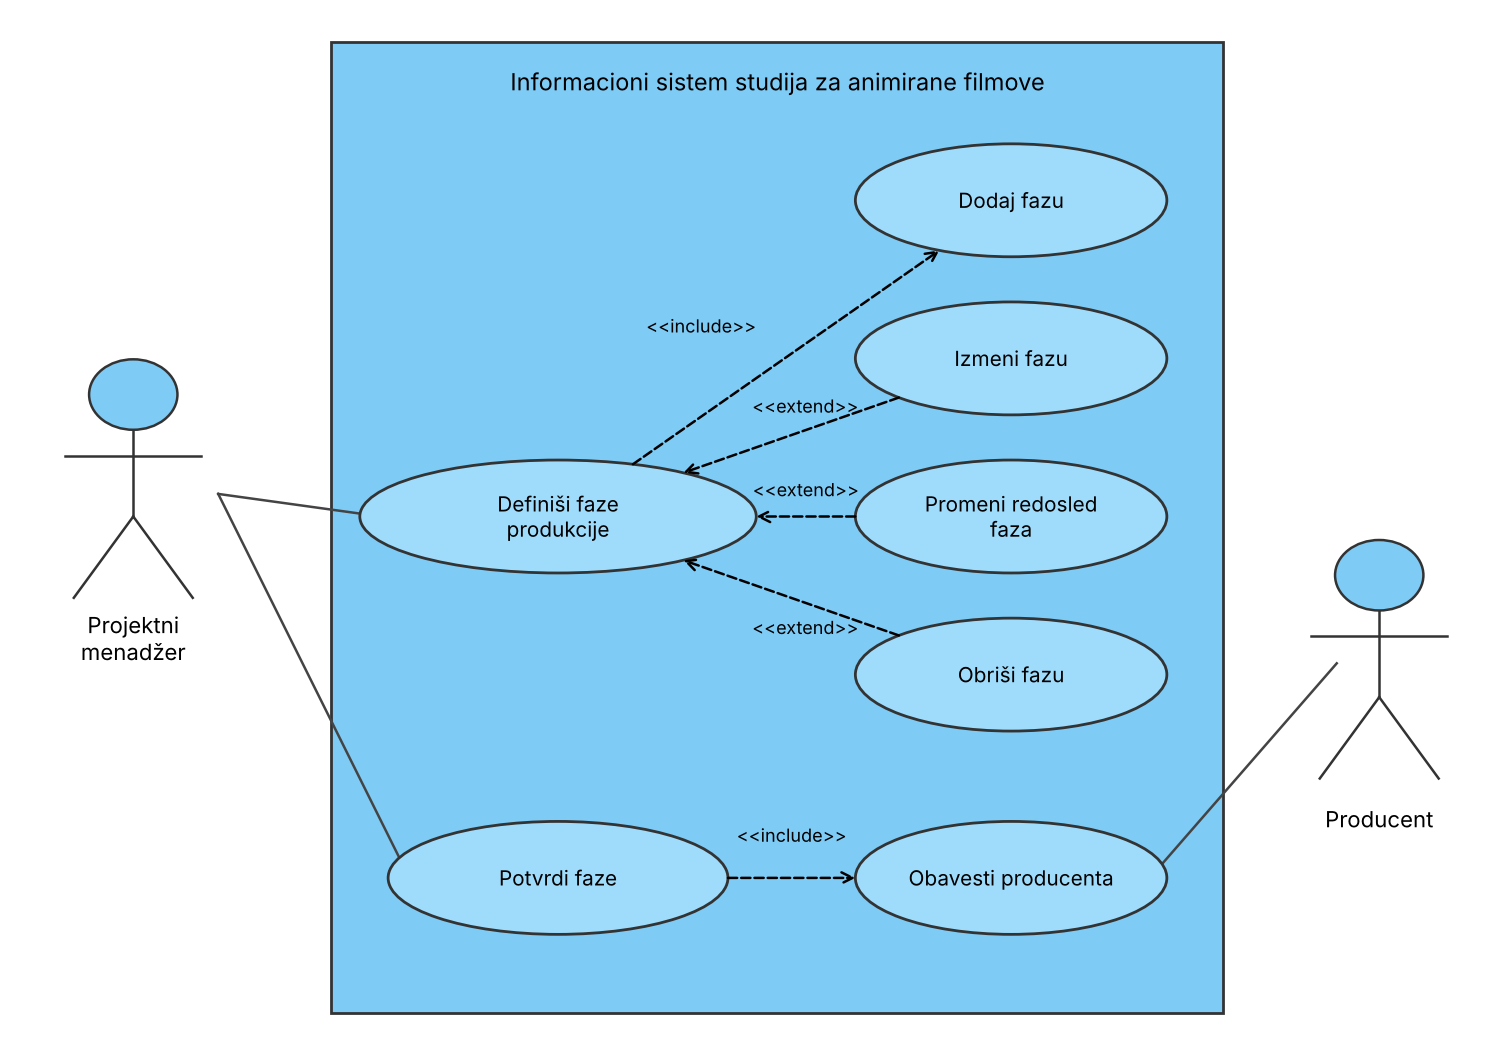
\includegraphics[width=\textwidth]{./dijagrami/dijagrami_slucajeva_upotrebe/definisanje_faza_produkcije.png}
	\caption{Dijagram slučaja upotrebe ,,Definisanje faza produkcije''}
 \end{figure}

\begin{figure}[H]
	\centering
	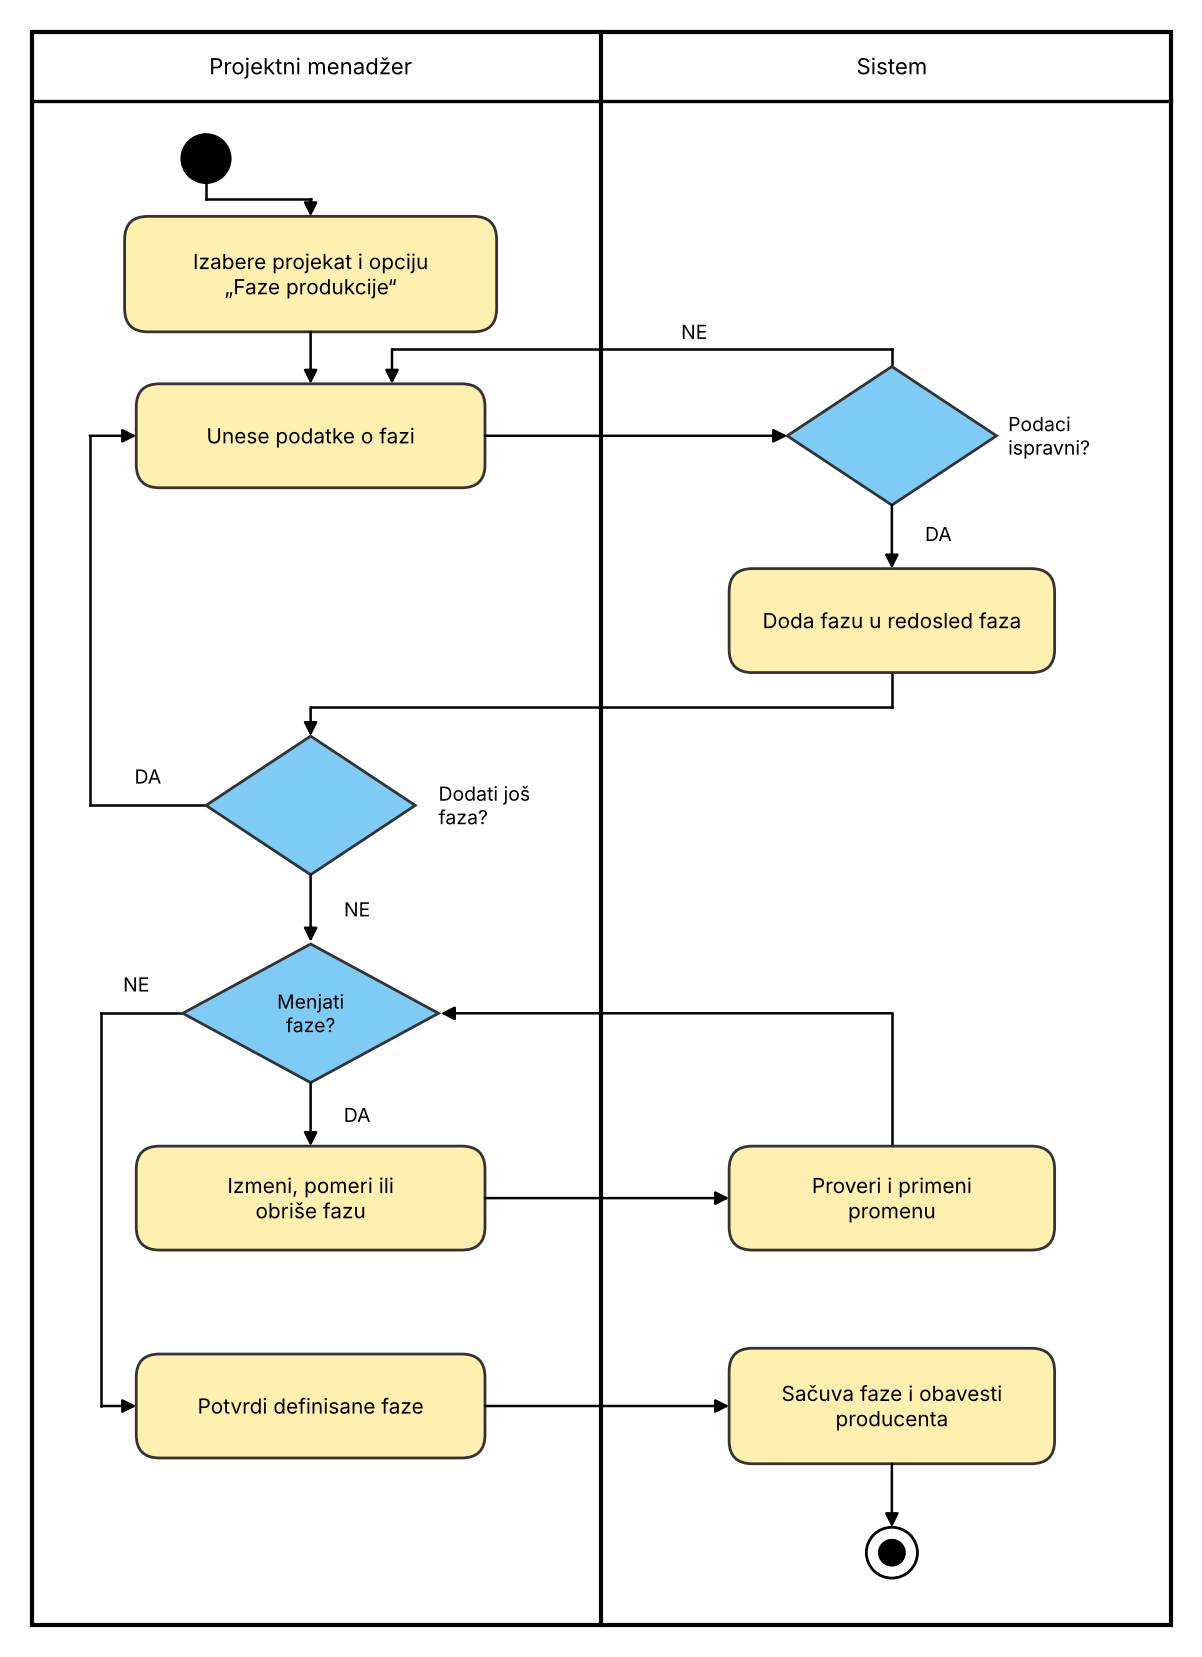
\includegraphics[width=\textwidth,height=0.8\textheight,keepaspectratio]{./dijagrami/dijagrami_aktivnosti/definisanje_faza_produkcije.png}
	\caption{Dijagram aktivnosti ,,Definisanje faza produkcije''}
 \end{figure}

\begin{figure}[H]
	\centering
	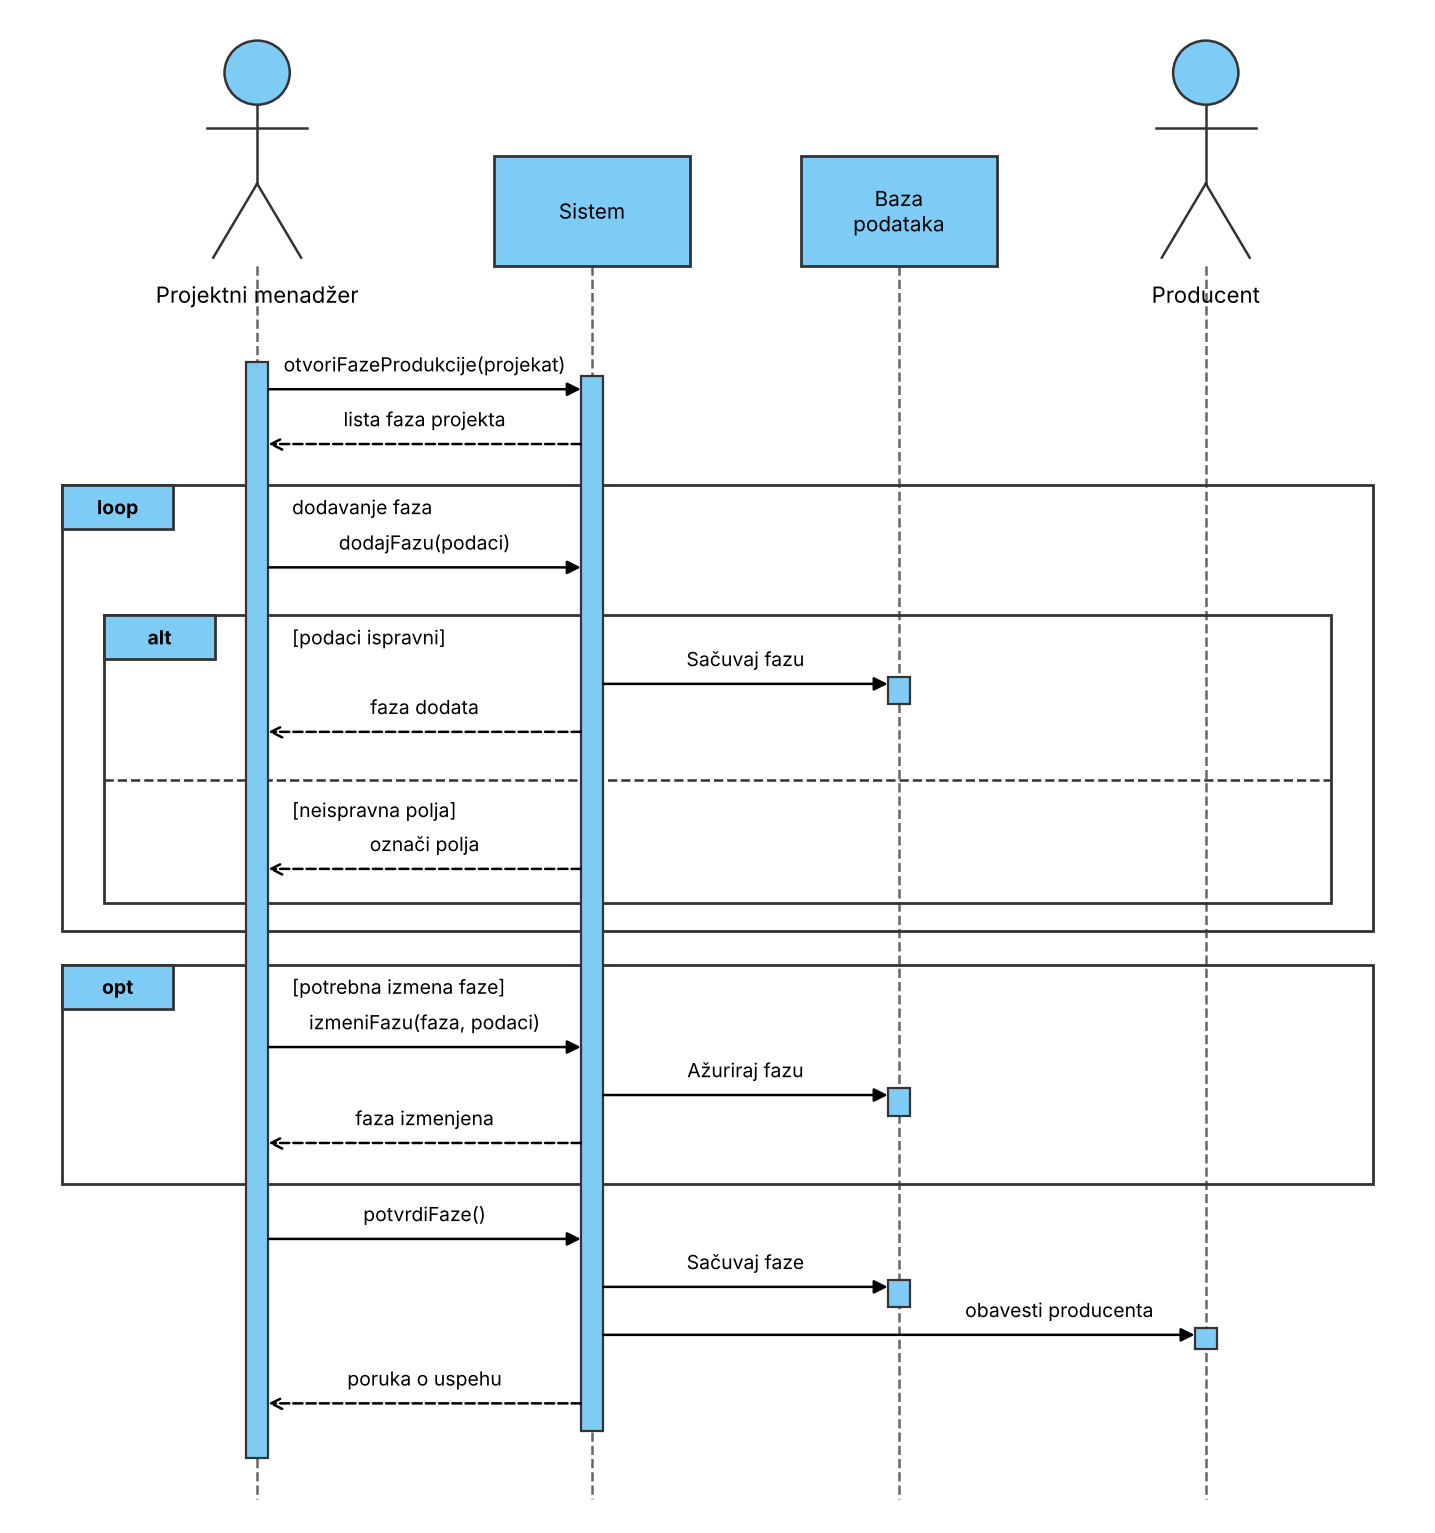
\includegraphics[width=\textwidth,height=0.8\textheight,keepaspectratio]{./dijagrami/dijagrami_sekvence/definisanje_faza_produkcije.png}
	\caption{Dijagram sekvence ,,Definisanje faza produkcije''}
 \end{figure}

\newpage
